\begin{frame}{Was müssen wir mindestens tun?}
\newcolumntype{C}[1]{>{\centering\let\newline\\\arraybackslash\hspace{0pt}}m{#1}}
\begin{tikzpicture}[->,>=stealth',shorten >=1pt,
  thick,main node/.style={circle,inner sep=1.5pt,fill=black!15,draw,font=\sffamily}, scale=1.15,
   pvs/.style={shape=rectangle, rounded corners,draw=issegrey!50,align=center}]
%%%%%%%%%%%%%%%%%% Orderings and embeddings

\node (t) at (4.3,6.5) {{$\top$}};
\node [text width=2.4cm](labelR) at ($(t)+(1,.7)$) {$\mathsf{P}$};

\node (r2) at ($(t)-(0.5,1)$) {{$\RN{2}$}};
\node (a2) at ($(t)-(-0.5,1)$) {{$2$}};

\node (r1) at ($(r2)-(0,1)$) {{$\RN{1}$}};
\node (a1) at ($(a2)-(0,1)$) {{$1$}};


\path[-,thin]
(r1) edge (r2)
     edge (a2)
(a1) edge (r2)
     edge (a2)
(a2) edge (t)
(r2) edge (t)
;      

  
   

%%%%%%%%%%%%%%%%%% SCSP problem
  \node[main node,minimum size = 12pt,text depth=.25ex,anchor=west,label=west:] (x) at (0,3) {$x$} ;
  \node[main node,minimum size = 12pt,text depth=.25ex,label=west:] (y) at ($(x)+(4.5,0)$) {$y$};  
  \node[main node,minimum size = 12pt,text depth=.25ex,label=east:] (z) at ($(x)+(9,0)$) {$z$};  
  \node[anchor=north west] (scsplabel) at ($(x)+(-.5,.7)$) {\color{issegrey} $SCSP$};

\node[pvs,dotted,text width=11.85cm,anchor=north west, text height=3.4cm] at ($(scsplabel.north west)+(-.3,0)$) {};
  \path[-,thin]
    (x) edge (y)
    (y) edge (z)
  ;
  \draw [thin,densely dashed,-] (x.south) -- ( $ (x.south) + (0,-.45)$); 
  \draw [thin,densely dashed,-] (y.south) -- ( $ (y.south) + (0,-.45)$);
  \draw [thin,densely dashed,-] (z.south) -- ( $ (z.south) + (0,-.45)$);   
  
  \node[anchor=north] (mux) at ($(x)+(0,-.5)$) {
\begin{tabular}{|c|c|}
  \hline 
  $x$ & $\mu_x$ \\ 
  \hline 
  0 & 1 \\ 
  1 & 2 \\ 
  \hline 
  \end{tabular}   
  };  
  
  \node[anchor=north] (muy) at ($(y)+(0,-.5)$) {
\begin{tabular}{|c|c|}
  \hline 
  $y$ & $\mu_y$ \\ 
  \hline 
  0 & 1 \\ 
  1 & 2 \\ 
  \hline 
  \end{tabular}   
  };  
  
    \node[anchor=north] (muz) at ($(z)+(0,-.5)$) {
\begin{tabular}{|c|c|}
  \hline 
  $z$ & $\mu_z$ \\ 
  \hline 
  0 & $\RN{2}$ \\ 
  1 & 1 \\ 
  \hline 
  \end{tabular}   
  };  
  
    \node[anchor=north] (muyx) at ($(x)+(2.25,-.5)$) {
\begin{tabular}{|c|c|c|}
  \hline 
  $x$ & $y$ & $\mu_{xy}$ \\ 
  \hline 
  0 & 0 & $\top$\\ 
  0 & 1 & $\RN{2}$\\ 
  1 & 0 & 2\\ 
  1 & 1 & 1\\  
  \hline 
  \end{tabular}   
  };  

    \node[anchor=north] (muyz) at ($(y)+(2.25,-.5)$) {
\begin{tabular}{|c|c|c|}
   \hline 
  $y$ & $z$ & $\mu_{yz}$ \\ 
  \hline 
  0 & 0 & $\RN{2}$\\ 
  0 & 1 & $\RN{1}$\\ 
  1 & 0 & $2$\\ 
  1 & 1 & 1\\ 
  \hline 
  \end{tabular}   
  };    
  
  \draw [thin,densely dashed,-] ($(muyx.north)+(0,.5)$) -- ($(muyx.north)+(0,-0.1)$);  
  
  \draw [thin,densely dashed,-] ($(muyz.north)+(0,.5)$) -- ($(muyz.north)+(0,-0.1)$);  
%\node[anchor=west] at (-.7, -3.5) { \textbf{Elimination order}:$\langle x, y, z \rangle$};

% |x| = \twopartdef { x } {x \geq 0} {-x} {x < 0}
%\node[anchor=west] at (-.7, -3.8) {\textbf{Embedding } into $\cSRngfree{\mathsf{R}}$: };

\end{tikzpicture}

\end{frame}

\begin{frame}{Von POs zu PVS: Skizze}

{
\Large
\begin{itemize}
\item Angenommen $(P, \leq_P)$ \pause 
\item Wir suchen eine PVS $(M, \cdot_M, \varepsilon_M, \leq_M)$ \pause
\item Wie \alert{Multiplikation} konstruieren?
\begin{itemize}
\item[-] Repräsentiere $p \in P$ durch ``sich selbst'': $p \in M$ $\checkmark$ \pause 
\item[-] Füge neue Elemente ``$p \cdot_M q$'' für alle Elemente $p,q \in M$ aus $\checkmark$ \pause
\item[-] Stelle sicher dass Kommutativität und Assoziativität gelten, nicht aber \emph{Idempotenz}: $(p \cdot_M q) \cdot_M r  = q \cdot_M (r \cdot_M p)$   \pause
\item[-] $\rightarrow$ Wähle \emph{Multimengen} über $P$ als Repräsentant der Produkte aus (Mengen \emph{wären} idempotent: $p \cdot_M p \neq p$ soll aber gelten. \pause
\item[-] Neutrales Element $\lbag \rbag$ für Multiplikation ``geschenkt''
\end{itemize}
\vspace*{2ex}
\pause
\item Welche Ordnungsbeziehungen \emph{müssen} gelten? \pause
\begin{itemize}
\item[-] Wenn $p \leq_P q$ dann $\lbag p \rbag \smytheq{P} \lbag q \rbag$ 
\item[-] $X \smytheq{P} \lbag  \rbag$, weil $\varepsilon_M$ das Maximum in $\leq_M$ sein soll
\item[-] Genannt: \alert{Smyth-Ordnung}
\end{itemize}
\item Beispiel: $\lbag 1, \RN{1}, 2 \rbag \smytheq{P} \lbag 2, \RN{2} \rbag$
\end{itemize}
}
\end{frame}

\begin{frame}{Was müssen wir mindestens tun?}

\begin{center} 
\newcolumntype{C}[1]{>{\centering\let\newline\\\arraybackslash\hspace{0pt}}m{#1}}
\begin{tikzpicture}[->,>=stealth',shorten >=1pt,
  thick,main node/.style={circle,inner sep=1.5pt,fill=black!15,draw,font=\sffamily}, scale=1.15,
   pvs/.style={shape=rectangle, rounded corners,draw=issegrey!50,align=center}]
%%%%%%%%%%%%%%%%%% Orderings and embeddings

\node (t) at (0.3,6.5) {{$\top$}};
\node [text width=2.4cm](labelR) at ($(t)+(1,.7)$) {$\mathsf{R}$};

\node (r2) at ($(t)-(0.5,1)$) {{$\RN{2}$}};
\node (a2) at ($(t)-(-0.5,1)$) {{$2$}};

\node (r1) at ($(r2)-(0,1)$) {{$\RN{1}$}};
\node (a1) at ($(a2)-(0,1)$) {{$1$}};


\path[-,thin]
(r1) edge (r2)
     edge (a2)
(a1) edge (r2)
     edge (a2)
(a2) edge (t)
(r2) edge (t)
;      

\draw [thin,dashed,-] ($(t)+(1.2,.5)$) -- ($(t)+(1.2,-5.5)$);
  
 % PVS<R>

\node [anchor=west,text width=5cm](labelPV) at ($(t)+(2.7,0.7)$) {$\PVSfree{\mathsf{R}}$};

\node (peps) at ($(t)+(3.25,0)$) {\color{isseorange} $\lbag \rbag$};
\node (pt) at ($(peps)-(0,1)$) {{$\lbag \top \rbag$}};
\node (pr2) at ($(pt)-(0.5,1)$) {{$\lbag \RN{2} \rbag$}};
\node (pa2) at ($(pt)-(-0.5,1)$) {{$\lbag 2 \rbag$}};

\node (pr1) at ($(pr2)-(0,1)$) {{$\lbag \RN{1} \rbag$}};
\node (pa1) at ($(pa2)-(0,1)$) {{$\lbag 1 \rbag$}};

\node (pr11) at ($(pr1)-(0,1)$) {\color{isseorange} $\lbag 1, \RN{1} \rbag$};
\node (pa11) at ($(pa1)-(0,1)$) {\color{isseorange} $\lbag 1, \RN{2} \rbag$};

\node (leftdots) at ($(pr1)-(1,1)$) {{\ldots}};
\node (rightdots) at ($(pa1)-(-1,1)$) {{\ldots}};

\node (downdots1) at ($(pr11)-(0,.75)$) {{\ldots}};
\node (downdots2) at ($(pa11)-(0,.75)$) {{\ldots}};

\path[-,thin]
(pr1) edge (pr2)
     edge (pa2)
(pa1) edge (pr2)
     edge (pa2)
(pa2) edge (pt)
(pr2) edge (pt)
(pt) edge (peps)
(pa11) edge (pa1)
(pr11) edge (pa1)
(pr11) edge (pr1)
(leftdots) edge (pr1)
(rightdots) edge (pa1)
(downdots1) edge (pr11)
(downdots2) edge (pa11)
;    
   
\end{tikzpicture}

\end{center}
\end{frame}



\begin{frame}{Looking for freedom \ldots} \small

\begin{center}
\begin{tikzpicture}[auto,->,
                    >=stealth',shorten >=1pt,thick,
                    node distance=.7cm,inner sep=2pt,
                    constraint/.style={circle,fill=black!15,draw,font=\sffamily\small},
                    bg/.style={shape=rectangle, rounded corners,
    draw, align=center,
    top color=white, bottom color=issegrey!15},
                    pvs/.style={shape=rectangle, rounded corners,
    draw=isseorange!50,fill=white, align=center}]
\node [anchor=west] at (0, .5) {$\mathrm{Cat}: \mathrm{POSet}$};
\node [anchor=west] at (0, -.5) {$\mathrm{Cat}: \mathrm{PVS}$};

\draw [dashed,-] (0,0) -- (11,0);

 \node[bg,text width=2.7cm, text height=1.5cm] at (5,1.6) {};
 \node[anchor=west] at (3.6,2.1) {$P$};
 
\node[constraint] (1) at (5, 2)                   {$\mathrm{c}_1$};
\node[constraint] (2) at ($ (1) + (-0.8, -0.8) $) {$\mathrm{c}_2$};  
\node[constraint] (3) at ($ (1) + ( 0.8, -0.8) $) {$\mathrm{c}_3$};  
%  
\path[every node/.style={font=\sffamily\tiny}]
  (2) edge (1)
  (3) edge (1)
  ;
 
\onslide<2-> { 
\node[pvs,text width=3.5cm,anchor=north west, text height=2.8cm] at (0.5,-1) {};
 \node[anchor=west] at (0.5,-1.3) {$\mathit{Weighted}(P)$};
  \node[anchor=west] at (0.5,-3.6) {$\langle \mathbb{N}, +, \geq, 0 \rangle$};
  
\node[constraint,label=west:2] (w1) at (2, -2)                   {$\mathrm{c}_1$};
\node[constraint,label=west:1] (w2) at ($ (w1) + (-0.8, -0.8) $) {$\mathrm{c}_2$};  
\node[constraint,label=west:1] (w3) at ($ (w1) + ( 0.8, -0.8) $) {$\mathrm{c}_3$};  
\node at (3.5, -2.3) {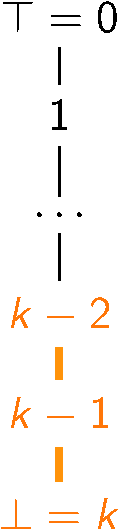
\includegraphics[width=.45cm]{img/search-space-weighted.pdf} }; 

%  
\path[every node/.style={font=\sffamily\tiny}]
  (w2) edge (w1)
  (w3) edge (w1)
  ;
}

\onslide<3->{
\draw [CornflowerBlue] (5,0.7) -- (2,-1);
\node [CornflowerBlue] at (4.2,-0.5) {$\mu(c) = \SPDw{}(c)$};
}  
 
\onslide<4->{
\node[pvs,text width=4.5cm,anchor=north west, text height=2.8cm] at (5.7,-1) {};
\node[anchor=west] at (5.7,-1.3) {$\mathit{PVS}\langle P \rangle $};
\node[anchor=west] at (5.7,-3.6) {$\langle \mathcal{M}^{\mathrm{fin}} (P), \mcup, \smytheq{P}, \lbag \rbag \rangle$};

\node[constraint,label=west:$\lbag \mathrm{c}_1 \rbag$] (p1) at (7, -2)                   {$\mathrm{c}_1$};
\node[constraint,label=east:$\lbag \mathrm{c}_2 \rbag$] (p2) at ($ (p1) + (-0.8, -0.8) $) {$\mathrm{c}_2$};  
\node[constraint,label=north:$\lbag \mathrm{c}_3 \rbag$] (p3) at ($ (p1) + ( 0.8, -0.8) $) {$\mathrm{c}_3$};  
\node at (9.2, -2.3) {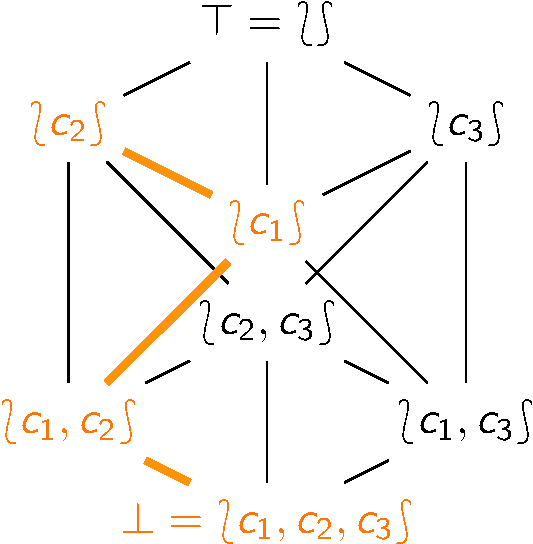
\includegraphics[width=2cm]{img/search-space.pdf} }; 
%  
\path[every node/.style={font=\sffamily\tiny}]
  (p2) edge (p1)
  (p3) edge (p1)
  ;
}
 
\onslide<5->{ 

\draw [isseorange] (5,0.7) -- (8,-1);
\node [isseorange] at (8.7,-0.5) {$\eta(c) = \lbag c \rbag$};
}

\onslide<6->{
\draw [issegrey] (5.7,-2) to [bend right] (4.2,-2);  
\node [issegrey] at (5,-1.5) {$(\SPDw{})^\#$};
}

\onslide<7->{
\draw [issegrey]  (4.2,-2.5) to [bend right] (5.7,-2.5);   
\node [issegrey] at (5,-3) {?};
}
\end{tikzpicture}
\end{center}

\end{frame}

\begin{frame}{Looking for freedom \ldots}
%\begin{itemize}
%\item (Konkrete) Kategorie $\mathsf{POSet}$: 
%\begin{itemize}
%\item[-] Objekte $\rightarrow$ partiell geordnete Mengen
%\item[-] Morphismen $\rightarrow$ monotone Funktionen
%\end{itemize}  
%\end{itemize}
\begin{lemma}[PVS-Freiheit \cite{knapp-schiendorfer2014}]
$\mathit{PVS}\langle P \rangle$ is the free partial valuation structure over the partial order $P$.
\end{lemma}


\begin{center}
\begin{tikzpicture}
  \matrix (m) [matrix of math nodes,row sep=3em,column sep=4em,minimum width=2em,ampersand replacement=\&]
  {
     P \& \mathit{PO}(\mathit{PVS}\langle P \rangle) \& \& \mathit{PVS}\langle P \rangle \\
      \& \mathit{PO}(M) \& \& M \\};
  \path[-stealth]
    (m-1-1) edge node [above] {$\eta_P^{\mathrm{PVS}}$} (m-1-2)
            edge node [below left] {$\varphi$} (m-2-2)
    (m-1-2) edge node [right] {$\mathit{PO}( \varphi^{\# \mathrm{PVS} })$} (m-2-2)
    (m-1-4) edge [dashed] node [right] {$\varphi^{\# \mathrm{PVS} }$} (m-2-4)
;
\end{tikzpicture}
\end{center}

\cemph{Freie Konstruktionen}

\begin{itemize}
\item no junk
\item no confusion
\end{itemize}
\end{frame}

\begin{frame}[fragile]{In MiniBrass}
\begin{lstlisting}
type FreePVS = PVSType<mset[maxOccurrences] of 1..maxP> = 
  params { 
    array[int, 1..2] of 1..nScs: orderRelation;
    int: maxP;
    int: maxPerSc;
    int: maxOccurrences :: default('mbr.nScs * mbr.maxPerSc');
  } in 
  instantiates with "../mbr_types/free-pvs-type.mzn" {
    times -> multiset_union;
    is_worse -> isSmythWorse;
    top -> {};
  };
\end{lstlisting}

\begin{lstlisting}
PVS: fp = new FreePVS("fp") {
   soft-constraint c1: 'embed(x == 4, 3, 3)';
   soft-constraint c2: 'embed(x in {1,3,4}, 2, 3)';
   soft-constraint c3: 'embed(x <= 3, 1, 3)';
   
   orderRelation : '[| 2, 1 | 3, 1 |]';
   maxP: '3' ;
   maxPerSc : '2';
}; 

solve fp;
\end{lstlisting}
\end{frame}

\begin{frame}{Smyth in MiniBrass}
Die Smyth-Ordnung haben wir induktiv definiert: 
\begin{align*}
& p <_P q \Rightarrow T \mcup \lbag p \rbag \smyth{P} T \mcup \lbag q \rbag \\
& T \supmset U \Rightarrow T \smyth{P} U 
\end{align*}


Wie können wir sie nun für einen Constraint-Solver codieren?

\pause 

\begin{lemma}[Witness für $\smytheq{P}$ \cite{schiendorfer2017}] \label{lem:inj-upper}
$T \smytheq{P} U$ gilt genau dann wenn es eine injektive
Abbildung $h : S(U) \to S(T)$ (genannt \emph{Witness}-Funktion) mit $p \leq_P q$ wenn
$h(j, q) = (k, p)$ für alle $(j, q) \in S(U)$ gibt. 
\end{lemma}

\vspace*{3ex}
\begin{center}

\begin{tikzpicture}
\begin{scope}[node distance = 0.8cm] 
\node (lbrac) at (0,0) {$\lbag$};
\node [fill=CornflowerBlue!30,circle,draw,right of = lbrac] (a) {$1$}; 
\node [fill=CornflowerBlue!30,circle,draw,right of = a] (b) {$\RN{1}$};
\node [fill=CornflowerBlue!30,circle,draw,right of = b] (c) {$2$};
\node [right of = c] (rbrac)  {$\rbag$};
\end{scope}

\node  [right of = rbrac]  (smyth)  {$\smytheq{P}$};

\begin{scope}[node distance = 0.8cm] 

\node [right of = smyth](rlbrac) {$\lbag$};
\node [fill=ForestGreen!20,circle,draw,right of = rlbrac] (ra) {$2$}; 
\node [fill=ForestGreen!20,circle,draw,right of = ra] (rb) {$\RN{2}$};
\node [right of = rb] (rrbrac)  {$\rbag$};

\path (ra) edge[thick,isseorange,bend left,->] (a)
  (rb) edge[thick,isseorange,bend right,->] (b)
  ;
  
\end{scope}

\end{tikzpicture}
\end{center}

\end{frame}